\documentclass{beamer}
% \usetheme{Frankfurt}
\usecolortheme{default}
% \usepackage{hyperref}
% \usepackage[utf8]{inputenc} % this is needed for german umlauts
% \usepackage[english]{babel} % this is needed for german umlauts
% \usepackage[T1]{fontenc}    % this is needed for correct output of umlauts in pdf

\usepackage{myStyle}

\begin{document}
\selectlanguage{english}

\title{\titleText}
%\subtitle{Pixelweise Klassifikation von Straße}
\author{\tutor}
\date{10. Juli 2015}
\subject{Machine Learning}

% \frame{\titlepage}

\begin{frame}{Was ist Machine Learning?}
    \begin{figure}[ht]
        \begin{minipage}[b]{0.45\linewidth}
            \centering
            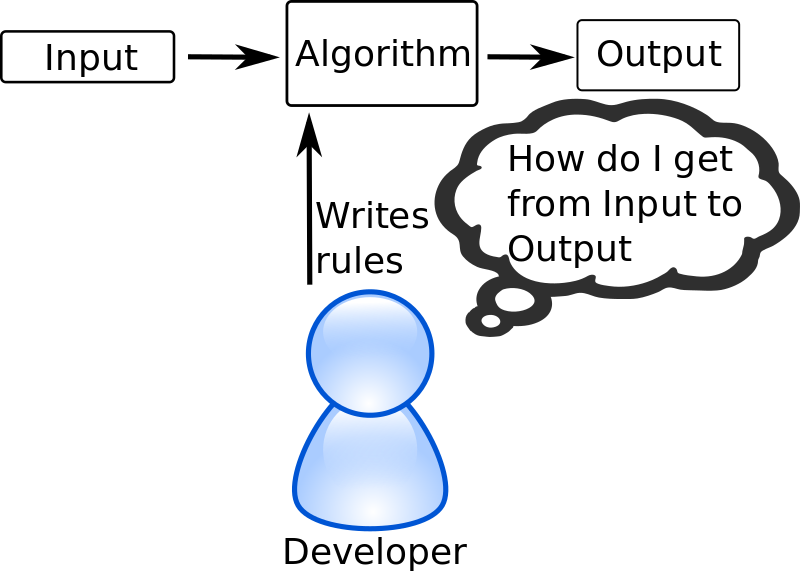
\includegraphics[width=\textwidth]{../images/traditional-model.png}
            \caption{Traditional Development Model}
        \end{minipage}
        \hspace{0.5cm}
        \begin{minipage}[b]{0.45\linewidth}
            \centering
            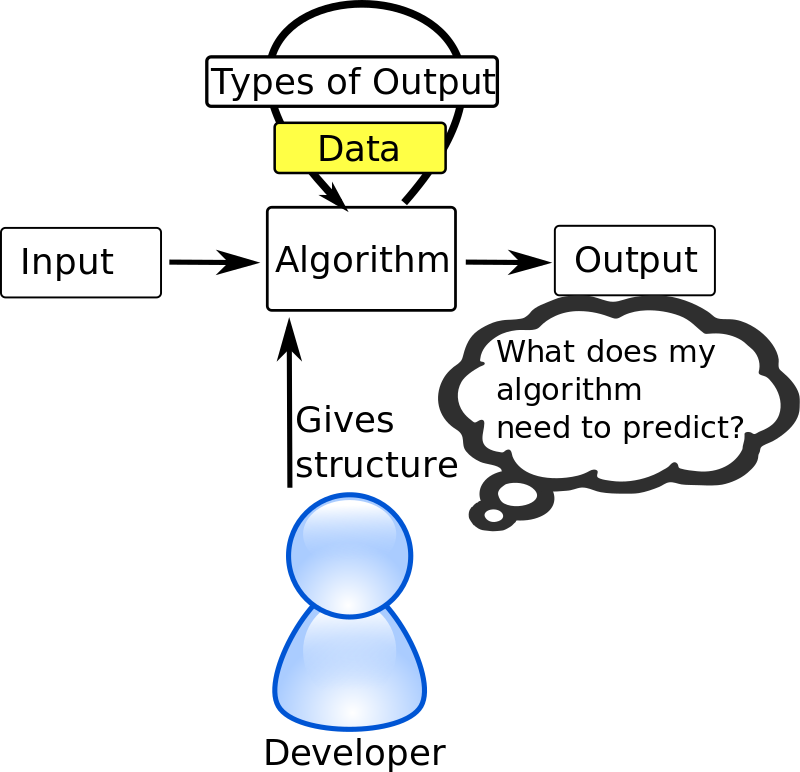
\includegraphics[width=\textwidth]{../images/ml-model.png}
            \caption{ML Model}
        \end{minipage}
    \end{figure}
\end{frame}

\begin{frame}{Was ist ML-KA?}
    \begin{itemize}
        \item Kurz für \textbf{Machine Learning Karlsruhe}
        \item (Inoffizielle) \textbf{Hochschulgruppe} seit 15.~Oktober 2015
        \item \textbf{Ziel}: Wissen über ML Verbreiten / Mehren
        \item \textbf{Idee}: Forum für interessierte Studenten bilden,
              organisation in kleinen Gruppen
        \item \textbf{Umsetzung} bisher
        \begin{itemize}
            \item Paper Discussion Group (PDG, wöchentlich)
            \item Teilnahme (und Preisträger) der Herbsttagung der Gesellschaft
                  für Datenanalyse und Numerische Klassifikation
        \end{itemize}
        \item Mehr auf \href{https://ml-ka.de/}{https://ml-ka.de}
    \end{itemize}
\end{frame}

\begin{frame}{Wer ist ML-KA?}
    \begin{itemize}
        \item Vorstand:
        \begin{itemize}
            \item Martin Thoma (info@martin-thoma.de)
            \item Marvin Teichmann
            \item Marvin Schweizer
        \end{itemize}
        \item Mitglieder: Überwiegend aktuelle Studenten des KIT
        \begin{itemize}
            \item 20~Mitglieder (Stand: 3. Februar 2016)
            \item 180 Facebook Mitglieder (Stand: 9. März 2016)
        \end{itemize}
    \end{itemize}
\end{frame}


\end{document}
